\section{Résultats expérimentaux}
	
	\subsection{Description des données}
		\paragraph{}Pour étudier les performances des algorithmes, nous utilisons six graphes du web présentés dans le tableau ci-dessous :
		
			\begin{center}\begin{tabular}{clrrr}
				\hline
				Graphe du web & nb noeuds & nb arcs & taille \\
				\hline
				wb-cs-stanford & 9 914 & 36 854 & 624 Ko \\
				Stanford & 281 903 & 2 312 497 & 37 Mo \\
				Stanford-Berkeley & 683 446 & 7 583 376 & 120 Mo \\
				in-2004 & 1 382 908 & 16 917 053 & 277 Mo \\
				wikipedia & 1 634 989 & 19 753 078 & 309 Mo \\
				wb-edu & 9 845 725 & 57 156 537 & 1.06 Go \\
				\hline
			\end{tabular}\end{center}
		
		\paragraph{}À la consultation de ce tableau, il est forcé de constater du volume que représente ces données, ce qui justifie le choix des implémentations qui a été fait.
		\paragraph{}Nous voudrions signaler que suite au téléchargement du fichier \textit{Stanford-Berkeley} le nombre de lignes indiquées dans le fichier n'est pas correct, $68344$ au lieu de $683446$.
		\paragraph{}Le code source est en \textbf{langage C}, le contrôle de l'utilisation correcte de la mémoire a été effectué à l'aide de l'option \textbf{-g} du compilateur \textbf{gcc} et l'outil d'exécution \textbf{valgrind}. Cependant, l'utilisation de ces outils décuplent le temps de calcul, nous avons donc préparer une deuxième version sans debug pour l'utiliser arès avoir vérifier l'utilisation correcte de la mémoire.
		
	\subsection{Mesures de performances}
	
		\paragraph{}Nous vous présentons dans un premier temps les résultats en temps et en itérations de l'implémentation de la méthode des puissances et de l'accélération de aitken.
		
			\begin{center}\begin{tabular}{lrrrrrrr}
				\hline
				Graphe du web & nb noeuds & nb arcs & taille & Puis (ité) & Puis (sec) & Aitk (ité) & Aitk (sec) \\
				\hline
				wb-cs-stanford & 9 914 & 36 854 & 624 Ko & 39 & < 1 & 37 & < 1 \\
				Stanford & 281 903 & 2 312 497 & 37 Mo & 52 & 2 & 53 & 2 \\
				Stanford-Berkeley & 683 446 & 7 583 376 & 120 Mo & 50 & 4 & 49 & 4 \\
				in-2004 & 1 382 908 & 16 917 053 & 277 Mo & 48 & 7 & 46 & 8 \\
				wikipedia & 1 634 989 & 19 753 078 & 309 Mo & 43 & 29 & 38 & 26 \\
				wb-edu & 9 845 725 & 57 156 537 & 1.06 Go & 47 & 44 & 52 & 50 \\
				\hline
			\end{tabular}\end{center}
			
		\paragraph{}La machine utilisée pour effectuer ces calculs possède un processeur Inter Core i7-7500U cadencé à 2.70GHz ainsi que 2 Go de RAM allouée pour la machine virtuelle sur laquelle se sont déroulés les programmes.
		
		\paragraph{}Il est aussi intéressant d'avoir un compte-rendu visuel pour comparer les méthodes. Les graphes ci-dessous représentent la valeur de $log(\| \Pi^{(k + 1)} - \Pi^{(k)} \|_{1})$ en fonction de l'itération $k$ pour les deux méthodes implémentées pour les six graphes du web. Ces courbes ont été réalisées à l'aide du logiciel \textit{GNUPLOT}.
		\paragraph{}On rappelle les constantes utilisées : $\alpha = 0.85$ et $\epsilon = 10^{-6}$. Les courbes ont été ajustées à la même échelle pour pouvoir les comparer de manière visuelle.\\
		
		\begin{minipage}[c]{.46\linewidth}
			\begin{center}
				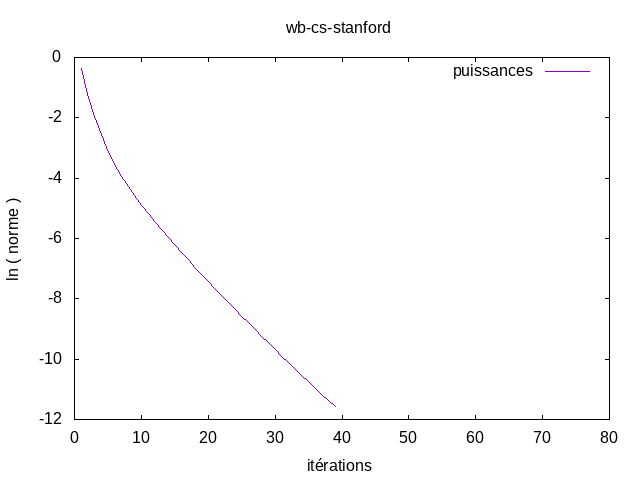
\includegraphics[scale=0.5]{plot-wb-cs-stanford.png}
			\end{center}
		\end{minipage} \hfill
		\begin{minipage}[c]{.46\linewidth}
			\begin{center}
				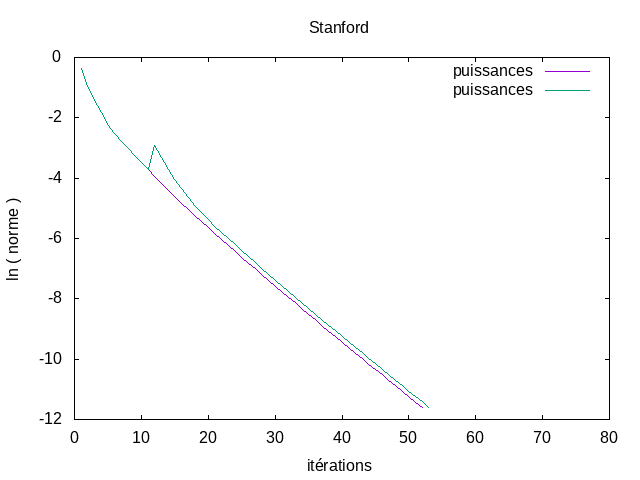
\includegraphics[scale=0.5]{plot-Stanford.png}
			\end{center}
		\end{minipage}\\
		\begin{minipage}[c]{.46\linewidth}
			\begin{center}
				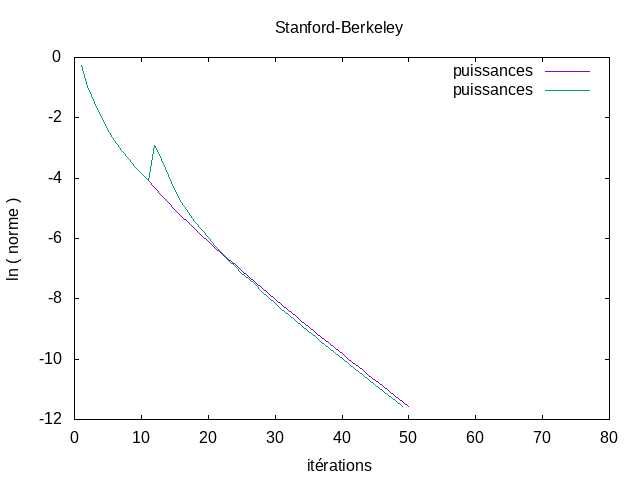
\includegraphics[scale=0.5]{plot-Stanford-Berkeley.png}
			\end{center}
		\end{minipage} \hfill
		\begin{minipage}[c]{.46\linewidth}
			\begin{center}
				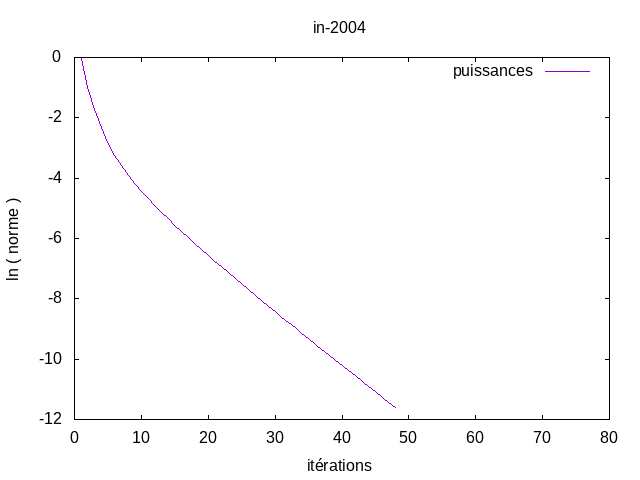
\includegraphics[scale=0.5]{plot-in-2004.png}
			\end{center}
		\end{minipage}\\
		\begin{minipage}[c]{.46\linewidth}
			\begin{center}
				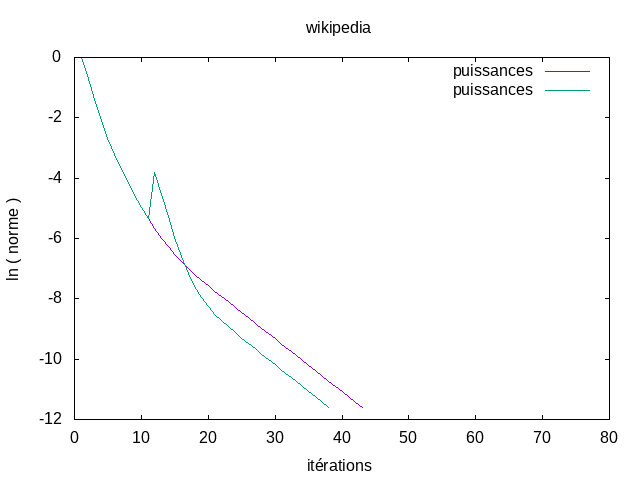
\includegraphics[scale=0.5]{plot-wikipedia.png}
			\end{center}
		\end{minipage} \hfill
		\begin{minipage}[c]{.46\linewidth}
			\begin{center}
				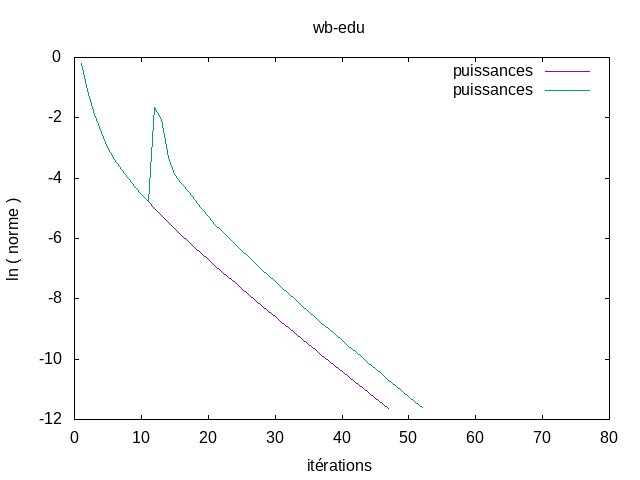
\includegraphics[scale=0.5]{plot-wb-edu.png}
			\end{center}
		\end{minipage}
		
		\paragraph{}Nous avons utilisé pour l'accélération de Aitken la version présentée dans le document \textit{Extrapolation Methods for Accelerating PageRank Computations} de Kamvar, Haveliwala, Manning et Golub provenant de l'université de Stanford.
		\paragraph{}Comme le document le préconise nous avons effectué une estimation de $\Pi$ à la $10^{e}$ itération, ce qui explique le pic du graphe. Cependant, les performances de l'accélération ne sont pas satisfaisantes pour les tests effectués.
		\paragraph{}Cela peut venir du fait que notre version de Aitken n'est pas correcte, en effet des résultats aberrants se produisent sous certaines conditions (voir fichier aitken.c), pour pallier à ce soucis nous ignorons la valeur aberrante et cela fausse les estimations faites.
